\documentclass[aspectratio=169,10pt,t,xcolor=table]{beamer}

% ---------- Theme ----------
\usetheme{default}
\usefonttheme{professionalfonts}
\setbeamertemplate{navigation symbols}{}
\definecolor{navy}{HTML}{002C5F}
\definecolor{sky}{HTML}{00AAD2}
\definecolor{sand}{HTML}{E4DCD3}
\definecolor{alert}{HTML}{D9381E}
\definecolor{ok}{HTML}{2E8B57}
\definecolor{ink}{HTML}{1E1E1E}
\definecolor{muted}{HTML}{6B7280}

\setbeamercolor{normal text}{fg=ink}
\setbeamercolor{frametitle}{fg=navy}
\setbeamercolor{title}{fg=white}
\setbeamercolor{structure}{fg=navy}
\setbeamercolor{itemize item}{fg=sky}
\setbeamercolor{itemize subitem}{fg=muted}
\setbeamercolor{block title}{bg=navy,fg=white}
\setbeamercolor{block body}{bg=sand!45}
\setbeamerfont{frametitle}{series=\bfseries,size=\Large}
\setbeamertemplate{itemize item}{\small$\blacktriangleright$}
\setbeamertemplate{itemize subitem}{\scriptsize$\bullet$}
\setbeamertemplate{blocks}[rounded]

\setbeamertemplate{frametitle}{%
  \vspace*{0.35cm}%
  {\color{sky}\rule{0.9cm}{3pt}}\par\vspace{3pt}%
  \insertframetitle\par\vspace{0.12cm}}
\setbeamersize{text margin left=0.8cm,text margin right=0.8cm}
\setbeamertemplate{footline}{%
  \leavevmode\hbox to\paperwidth{%
    \hspace{0.4cm}{\tiny\color{muted}Honk-Sense \,|\, HCoE Mobility Innovation Ideathon 2026 \,|\, Topic 1: India-Smart Interaction}%
    \hfill{\tiny\color{navy}\textbf{\insertframenumber}}\hspace{0.4cm}}\vspace{0.12cm}}

% ---------- Packages ----------
\usepackage{tikz}
\usetikzlibrary{arrows.meta,positioning,shapes.geometric,calc,fit,backgrounds}
\usepackage{booktabs}
\usepackage{tabularx}
\usepackage{amsmath}
\usepackage{xcolor}
\usepackage{xurl}
\usepackage{pifont}
\newcommand{\yes}{\textcolor{ok}{\ding{51}}}
\newcommand{\no}{\textcolor{muted!60}{--}}
\newcommand{\partly}{\textcolor{orange}{\small$\sim$}}
\newcolumntype{Y}{>{\raggedright\arraybackslash}X}
\renewcommand{\arraystretch}{1.18}

\newcommand{\hl}[1]{\textcolor{navy}{\textbf{#1}}}
\newcommand{\src}[1]{{\tiny\color{muted}#1}}
\newcommand{\bignum}[2]{%
  \begin{minipage}[t]{\linewidth}\centering
    {\fontsize{26}{28}\selectfont\color{alert}\textbf{#1}}\\[2pt]
    {\small #2}
  \end{minipage}}


% use-case card: image, title, rating colour, rating, body
\newcommand{\usecase}[5]{%
  \begin{minipage}[t]{\linewidth}
  \includegraphics[width=\linewidth]{img/#1}\par\vspace{2pt}
  {\normalsize\bfseries\color{navy}#2}\par\vspace{2pt}
  \footnotesize\raggedright #5
  \end{minipage}}
\newcommand{\honest}[1]{\par\vspace{2pt}{\color{muted}\textbf{Honest limit:} #1}}

\title{Honk-Sense}
\subtitle{A car that understands Indian roads by ear}
\author{Piyush Anand \and Ankith Deegoju}
\institute{IIT Hyderabad}
\date{HCoE Mobility Innovation Ideathon 2026 \,\textbullet\, Topic 1: India-Smart Interaction}

\begin{document}

% ================= TITLE =================



{
\setbeamertemplate{footline}{}
\begin{frame}[plain]
\begin{tikzpicture}[remember picture,overlay]
  \fill[navy] (current page.south west) rectangle (current page.north east);
  \fill[sky] ([yshift=-1.2cm]current page.north west) rectangle ++(0.35,-3.4);
  % sound waves motif
  \foreach \r/\o in {1.2/0.55,2.0/0.4,2.8/0.28,3.6/0.16}{
    \draw[sky,line width=2pt,opacity=\o] ([xshift=-2.6cm,yshift=-0.2cm]current page.east) ++(160:\r) arc (160:200:\r);}
  \fill[white] ([xshift=-2.6cm,yshift=-0.2cm]current page.east) circle (0.32);
  \node[anchor=north west,text width=11cm,white] at ([xshift=1cm,yshift=-1.25cm]current page.north west) {%
    {\fontsize{38}{40}\selectfont\bfseries Honk-Sense}\\[6pt]
    {\Large A car that understands Indian roads by ear}\\[18pt]
    {\normalsize Directional alerts for the horns and sirens that matter.\\
    Silence for everything else.}};
  \node[anchor=south west,text width=14cm,white] at ([xshift=1cm,yshift=0.9cm]current page.south west) {%
    \small Piyush Anand \quad\textbullet\quad Ankith Deegoju \quad\textbullet\quad IIT Hyderabad\\[3pt]
    \color{sky}\footnotesize HCoE Mobility Innovation Ideathon 2026 \textbullet\ Topic 1: India-Smart Interaction \textbullet\ Track A};
\end{tikzpicture}
\end{frame}
}

% ================= PROBLEM =================
\begin{frame}{The Problem: Loud Roads, Deaf Cabins}
\begin{columns}[T]
\begin{column}{0.32\textwidth}
\bignum{\textgreater 90 dB}{daily honking exposure for Mumbai commuters (IIT Bombay study)}
\end{column}
\begin{column}{0.32\textwidth}
\bignum{\textgreater 100 dBA}{two-wheeler horns measured at 3 m in Mumbai (MPCB)}
\end{column}
\begin{column}{0.32\textwidth}
\bignum{25--35 min}{for ambulances to reach accident scenes on core national highways}
\end{column}
\end{columns}
\vspace{4pt}
\begin{itemize}\small
  \item \hl{Alert fatigue:} drivers hear so many honks that they tune \emph{all} of them out, including the few that signal real danger.
  \item \hl{The cabin paradox:} better insulation, closed windows, AC and music make modern cabins quieter, so sirens and nearby horns are heard \emph{later}.
  \item \hl{No sense of direction:} even when a driver hears a siren, it is hard to tell where it is coming from in dense traffic.
  \item \hl{Ambulances lose time:} drivers notice them late and do not know which way to move.
\end{itemize}
\end{frame}

% ================= DATA (research) =================
\begin{frame}{What the Data Says}
\begin{columns}[T]
\begin{column}{0.48\textwidth}
\bignum{4.8 lakh}{road accidents in 2023; 1.72 lakh deaths}
\end{column}
\begin{column}{0.48\textwidth}
\bignum{36\%}{rear-end (21\%) + side (15\%) collisions}
\end{column}
\end{columns}
\vspace{14pt}
\begin{block}{What We Claim}
\begin{itemize}\small
  \item \hl{14--31\% improvement} from awareness systems in similar situations: blind-spot monitoring cut lane-change crashes by 14\% (IIHS), and side blind-zone alerts cut lane changes made without a mirror check by 31\%.
  \item We do not claim a number for Honk-Sense yet.
\end{itemize}
\end{block}
\end{frame}

% ================= WHY ACCIDENTS STILL HAPPEN (research) =================
\begin{frame}{Why Accidents Still Happen Despite Existing Systems}
\vspace{-0.15cm}
{\small\textbf{The problem:} important sounds outside the car do not reach the driver in a usable form: on time, with a direction, and separated from the noise.}
\vspace{4pt}
\begin{columns}[T]
\begin{column}{0.48\textwidth}
\begin{itemize}\footnotesize
  \item \textbf{Mirrors depend on attention.} Drivers do not check them, or check and fail to register: 75\% of lane-change crashes involve this recognition failure.
  \item \textbf{Blind-spot systems are not universal.} Radar BSM is mostly on upper variants, and tuned for orderly lanes, not weaving two-wheelers.
  \item \textbf{Every sensor needs line of sight.} Nothing sees around a bus, a truck or a hairpin bend.
\end{itemize}
\end{column}
\begin{column}{0.48\textwidth}
\begin{itemize}\footnotesize
  \item \textbf{Proximity sensors are short-range.} Ultrasonic sensors reach about 2\,m and are made for parking.
  \item \textbf{Sirens lose to the cabin.} Sealing, AC and music cut them down; drivers placed a siren correctly only 26\% of the time.
  \item \textbf{Too many horns means no horn.} Habituation makes the meaningful honk invisible.
\end{itemize}
\end{column}
\end{columns}
\vspace{3pt}

\begin{tikzpicture}
  \node[fill=navy,text=white,rounded corners=4pt,text width=\dimexpr\textwidth-16pt\relax,align=center,inner sep=5pt,font=\small] {\textbf{Gap:} turning outside sound into a short, directional, filtered cue inside the car.};
\end{tikzpicture}
\vfill
\src{Sources: FMCSA (lane-change recognition failure); US DOT siren audibility study; TI SPRY331 (ultrasonic range); SAE 2026-26-0035 (ADAS in India). Full links on References (2).}
\end{frame}

% ================= PITCH =================
\begin{frame}{Honk-Sense in One Slide}
\vspace{-0.3cm}
\begin{columns}[T]
\begin{column}{0.56\textwidth}
\begin{block}{The idea}
Exterior microphones and an on-board AI \hl{classify every road sound}, \hl{locate where it comes from}, and decide whether the people inside need to know.
\end{block}
\vspace{2pt}
\begin{itemize}\small
  \item \textbf{Ambulance behind?} Music dips, a rear chime plays: \emph{``Ambulance behind, keep left''}.
  \item \textbf{Bike honking in the blind spot?} A chime from that side, plus an arrow.
  \item \textbf{Routine honking in a jam?} \hl{Nothing.} The cabin stays calm.
  \item \textbf{Fleet:} cars that hear a siren warn Hyundai cars ahead.
\end{itemize}
\end{column}
\begin{column}{0.4\textwidth}
\centering
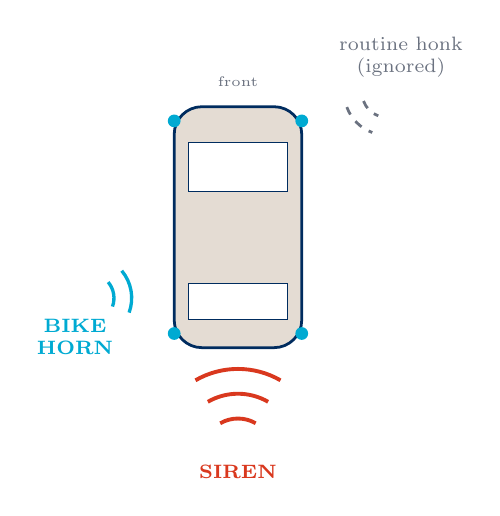
\begin{tikzpicture}[scale=0.9,baseline=(current bounding box.north)]
  % car top view
  \draw[rounded corners=10pt,fill=sand,draw=navy,line width=1pt] (-0.9,-1.7) rectangle (0.9,1.7);
  \draw[fill=white,draw=navy] (-0.7,0.5) rectangle (0.7,1.2);
  \draw[fill=white,draw=navy] (-0.7,-1.3) rectangle (0.7,-0.8);
  \foreach \p in {(-0.9,1.5),(0.9,1.5),(-0.9,-1.5),(0.9,-1.5)} \fill[sky] \p circle (0.09);
  % ambulance waves from behind
  \foreach \r in {0.5,0.85,1.2}\draw[alert,line width=1.4pt] (0,-3.2) ++(60:\r) arc (60:120:\r);
  \node[alert,font=\scriptsize\bfseries] at (0,-3.45) {SIREN};
  % bike horn from rear-left
  \foreach \r in {0.35,0.6}\draw[sky,line width=1.2pt] (-2.1,-1.0) ++(-20:\r) arc (-20:40:\r);
  \node[sky,font=\scriptsize\bfseries,align=center] at (-2.3,-1.55) {BIKE\\HORN};
  % ignored honk
  \foreach \r in {0.35,0.6}\draw[muted,line width=1pt,dashed] (2.1,1.9) ++(200:\r) arc (200:250:\r);
  \node[muted,font=\scriptsize,align=center] at (2.3,2.4) {routine honk\\(ignored)};
  \node[font=\tiny,muted] at (0,2.05) {front};
\end{tikzpicture}
\end{column}
\end{columns}
\end{frame}

% ================= COMPARISON (research) =================
\begin{frame}{Comparison with Existing Technologies}
\vspace{-0.1cm}
\small\renewcommand{\arraystretch}{1.16}
\setlength{\tabcolsep}{4pt}
\rowcolors{2}{sand!35}{white}
\begin{tabularx}{\textwidth}{@{}Y*{6}{>{\centering\arraybackslash}p{1.38cm}}@{}}
\toprule
\rowcolor{white}\textbf{Situation} & \textbf{Mirrors} & \textbf{Dashcam} & \textbf{Ultra\-sonic} & \textbf{Radar BSM} & \textbf{Camera ADAS} & \cellcolor{navy}\textcolor{white}{\textbf{Honk-Sense}} \\
\midrule
Ambulance hidden in traffic & \no & \no & \no & \no & \no & \yes \\
Horn behind a blind turn & \no & \no & \no & \no & \no & \yes \\
Which side a horn came from & \no & \no & \no & \no & \no & \yes \\
Honking bike in blind spot & \partly & \no & \no & \yes & \no & \yes \\
\emph{Silent} car in blind spot & \partly & \no & \no & \yes & \no & \no \\
Parking, low-speed obstacles & \partly & \no & \yes & \no & \partly & \no \\
Lane departure, car ahead & \no & \no & \no & \no & \yes & \no \\
Evidence after a crash & \no & \yes & \no & \no & \no & \no \\
\bottomrule
\end{tabularx}
\rowcolors{1}{}{}
\vspace{1pt}
{\scriptsize\color{muted}\yes\ does it \quad \partly\ partly \quad \no\ cannot}\par
\vspace{3pt}

\begin{tikzpicture}
  \node[fill=navy,text=white,rounded corners=4pt,text width=\dimexpr\textwidth-16pt\relax,align=center,inner sep=5pt,font=\small] {Other systems need line of sight. Only Honk-Sense brings a horn's intent into the cabin, with a direction.};
\end{tikzpicture}
\end{frame}

% ================= BEHAVIOUR =================
\begin{frame}{The Horn as a Language on Indian Roads}
\vspace{-0.3cm}
\begin{columns}[T]
\begin{column}{0.48\textwidth}
\begin{block}{On Indian roads, the horn is a language}
\begin{itemize}\small
  \item \textbf{``I'm here''}: a bike announcing itself in your blind spot
  \item \textbf{``I'm overtaking''}: trucks invite it with \emph{``Horn OK Please''} painted on the back
  \item \textbf{``Careful, blind turn''}: hill roads have \emph{``Blow Horn''} signs
  \item \textbf{``Move''} or \textbf{``signal is green''}: impatience in jams
  \item \textbf{Siren}: give way now
\end{itemize}
\end{block}
\end{column}
\begin{column}{0.48\textwidth}
\begin{block}{How drivers respond}
\begin{itemize}\small
  \item \textbf{Habituation:} so many honks that \emph{all} are ignored, including the important ones
  \item \textbf{Sealed cabins:} windows up, AC and music on, so outside sounds arrive late
  \item \textbf{Direction confusion:} a siren is heard, but not from where; drivers freeze or move the wrong way
  \item \textbf{Hearing gaps:} elderly and hearing-impaired drivers rely on mirrors alone
\end{itemize}
\end{block}
\end{column}
\end{columns}
\vspace{14pt}
\centering\small The car should understand this language the way an experienced Indian driver does, and \hl{translate only what matters}.
\end{frame}

% ================= TOPIC FIT =================
\begin{frame}{Why This Answers India-Smart Interaction}
\begin{block}{Question}
\emph{How can vehicles understand and interact with Indian users more naturally?}
\end{block}
\vspace{6pt}
Honk-Sense extends ``understanding'' from the \hl{user's voice} to the \hl{user's environment}:
\begin{itemize}
  \item understands India-specific sounds: two-wheeler horns, auto-rickshaw horns, pressure horns, Indian siren patterns;
  \item interacts naturally: the right speaker, the right moment, in the user's language.
\end{itemize}
\vspace{10pt}

\begin{tikzpicture}
  \node[fill=navy,text=white,rounded corners=4pt,text width=\dimexpr\textwidth-16pt\relax,align=center,inner sep=6pt,font=\normalsize] {Voice assistants understand what you say. Honk-Sense understands what the road is saying.};
\end{tikzpicture}
\end{frame}

% ================= BEFORE AFTER =================
\begin{frame}{A Drive with and without Honk-Sense}
\vspace{4pt}
\small\renewcommand{\arraystretch}{1.24}
\begin{tabularx}{\textwidth}{@{}p{3.6cm}YY@{}}
\toprule
\textbf{Moment} & \textbf{Today} & \textbf{With Honk-Sense} \\
\midrule
Stuck in a honking jam & Constant noise and stress; every honk ignored & \textcolor{ok}{\textbf{Calm cabin.}} Nothing is announced \\
Bike honks during a lane change & A horn somewhere; driver unsure where & Chime from the \textbf{left} speakers and a left arrow \\
Ambulance 200 m behind, music on & Noticed late; driver freezes & Music dips: \emph{``Ambulance behind, keep left''} \\
Ambulance 1 km behind & No idea it is coming & Fleet notice: \emph{``Ambulance approaching, about 1 minute''} \\
Truck overtaking on a highway & Pressure horn startles the family & Soft cue: \emph{``Truck overtaking on the right''} \\
Hearing-impaired driver & Misses sirens entirely & Arrow on the cluster and a seat vibration \\
\bottomrule
\end{tabularx}

\end{frame}

% ================= SOLUTION OVERVIEW =================
\begin{frame}{The Experience in Four Steps}
\vspace{8pt}
\centering
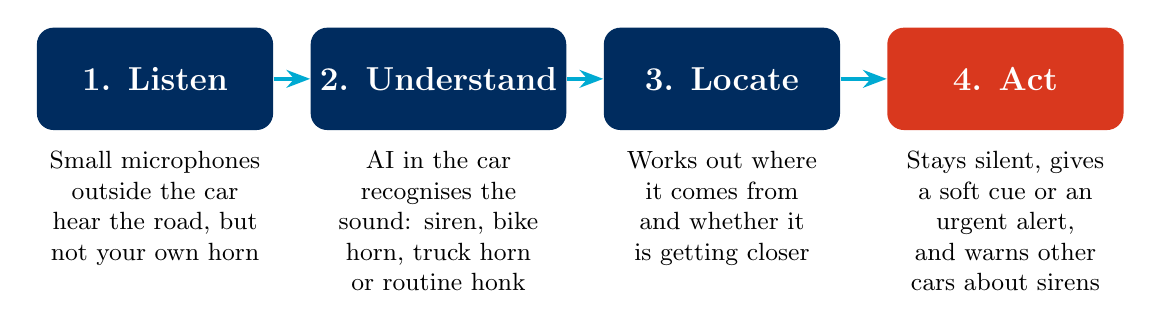
\begin{tikzpicture}[
  stage/.style={rectangle,rounded corners=6pt,fill=navy,text=white,minimum width=3.0cm,minimum height=1.3cm,font=\large\bfseries},
  desc/.style={text width=3.0cm,font=\small,align=center},
  arr/.style={-{Stealth[length=3mm]},line width=1.4pt,sky}]
  \node[stage] (l) at (0,0) {1. Listen};
  \node[stage] (u) at (3.6,0) {2. Understand};
  \node[stage] (o) at (7.2,0) {3. Locate};
  \node[stage,fill=alert] (a) at (10.8,0) {4. Act};
  \draw[arr] (l) -- (u); \draw[arr] (u) -- (o); \draw[arr] (o) -- (a);
  \node[desc,below=4pt of l] {Small microphones outside the car hear the road, but not your own horn};
  \node[desc,below=4pt of u] {AI in the car recognises the sound: siren, bike horn, truck horn or routine honk};
  \node[desc,below=4pt of o] {Works out where it comes from and whether it is getting closer};
  \node[desc,below=4pt of a] {Stays silent, gives a soft cue or an urgent alert, and warns other cars about sirens};
\end{tikzpicture}
\vspace{16pt}
\begin{block}{Silence is a feature}
The car stays \textbf{quiet} for everyday honks and speaks up \textbf{only when it matters}.
\end{block}
\vspace{8pt}
\end{frame}

% ================= USE CASES (research) =================
\begin{frame}{Use Cases (1/3): Emergencies and Horn Direction}
\vspace{-0.3cm}
\begin{columns}[T]
\begin{column}{0.47\textwidth}
\usecase{u1_ambulance.jpg}{U1. Hidden ambulance}{ok}{STRONG}{%
An ambulance is behind a bus; music on, windows up. Honk-Sense shows \emph{``Ambulance, behind left, approaching''}, dips the music and suggests which way to move.}
\end{column}
\begin{column}{0.47\textwidth}
\usecase{u2_bikes.jpg}{U2. Which horn, and where?}{ok}{STRONG}{%
Horns from every side; one is a bike at your rear-left as you turn left. Honk-Sense shows only the horns that are close and directed at you, with an arrow, and ignores the rest.}
\end{column}
\end{columns}
\vfill
\src{Photos: Wikimedia Commons. U1: Biswarup Ganguly (CC BY 3.0); U2: Amityadav8 (public domain).}
\end{frame}

\begin{frame}{Use Cases (2/3): Blind Spots and Blind Turns}
\vspace{-0.3cm}
\begin{columns}[T]
\begin{column}{0.47\textwidth}
\usecase{u3_blowhorn.jpg}{U3. Honk in the blind spot}{orange}{MEDIUM}{%
A bike or truck in your blind spot honks before you change lanes; most cars in India have no radar blind-spot monitor. Honk-Sense: \emph{``Horn, right rear''} as you signal.}
\end{column}
\begin{column}{0.47\textwidth}
\usecase{u4_hairpin.jpg}{U4. Around the bend}{ok}{STRONG}{%
A bus honks at a hairpin bend before it is in view. Honk-Sense warns \emph{``Vehicle ahead, around the bend''} seconds earlier.\par\vspace{2pt}
Cameras and radar cannot see around the corner; sound can.}
\end{column}
\end{columns}
\vfill
\src{Photos: Wikimedia Commons. U3: Justin Morgan (CC BY-SA 2.0); U4: Rohini (CC BY-SA 3.0).}
\end{frame}

\begin{frame}{Use Cases (3/3): A Calmer Cabin}
\vspace{-0.3cm}
\begin{columns}[T]
\begin{column}{0.5\textwidth}
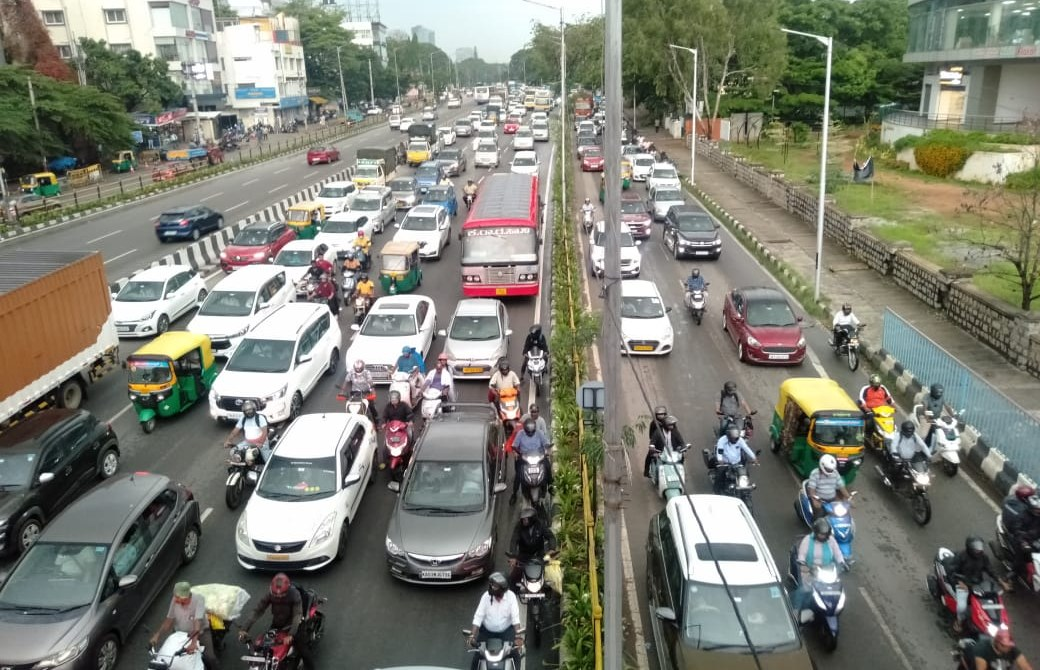
\includegraphics[width=\linewidth]{img/u6_jam.jpg}
\end{column}
\begin{column}{0.46\textwidth}
{\Large\bfseries\color{navy}U5. Fewer interruptions}\par\vspace{10pt}
\small
\begin{itemize}
  \item Peak-hour traffic, with street noise above 90--100\,dB.
  \item Drivers hear so many horns that they stop reacting to all of them.
  \item Less stress, and less alarm fatigue.
\end{itemize}
\end{column}
\end{columns}
\vfill
\src{Photo: Wikimedia Commons. Divya Chinnasamy (CC0).}
\end{frame}

% ================= HMI =================
\begin{frame}{In-Cabin Experience: Three Alert Tiers}
\small\renewcommand{\arraystretch}{1.05}
\begin{tabularx}{\textwidth}{@{}p{1.9cm}p{4.0cm}YY@{}}
\toprule
\textbf{Tier} & \textbf{Triggered by} & \textbf{What the driver gets} & \textbf{What passengers get} \\
\midrule
\textcolor{muted}{\textbf{0. Silent}} & Routine honks, distant horns, sounds ahead in a jam & Nothing (logged only) & Nothing \\
\textcolor{sky}{\textbf{1. Aware}} & Horn very close at the side or rear; truck overtaking & Short directional chime from the matching speaker; arrow icon on the cluster & Nothing \\
\textcolor{alert}{\textbf{2. Urgent}} & Siren approaching; horn plus fast approach during a lane change & Music ducked, spoken cue in the driver's language, arrow and suggested action & Rear-screen banner: \emph{``Ambulance approaching''} \\
\bottomrule
\end{tabularx}
\vspace{2pt}
\footnotesize
\begin{columns}[T]
\begin{column}{0.48\textwidth}
\textbf{Spatial audio cue}\\
The chime plays from the speaker nearest the sound source, so the driver's ears point the right way \emph{before} they read anything.
\end{column}
\begin{column}{0.48\textwidth}
\textbf{Accessibility}\\
Hearing-impaired mode: visual and seat-haptic alerts only. Volume, languages and tiers are configurable per driver profile.
\end{column}
\end{columns}
\end{frame}

% ================= FLEET =================
\begin{frame}{Fleet Layer: Clearing the Way for Ambulances}
\vspace{-0.3cm}
\begin{columns}[c]
\begin{column}{0.55\textwidth}
\begin{enumerate}\small
  \item A Hyundai car hears a siren and estimates its direction of travel.
  \item It shares only four facts with Hyundai's connected-car cloud: a siren was heard, where, which way it is heading, and when.
  \item The cloud confirms the event when several cars report it, which filters false alarms.
  \item Hyundai cars \textbf{ahead on the same road} get an early notice: \emph{``Ambulance approaching from behind in about 1 minute. Prepare to keep left.''}
\end{enumerate}
\vspace{3pt}
{\footnotesize\textbf{Future:} with city emergency services, the same channel could carry official ambulance routes.}
\end{column}
\begin{column}{0.42\textwidth}
\centering
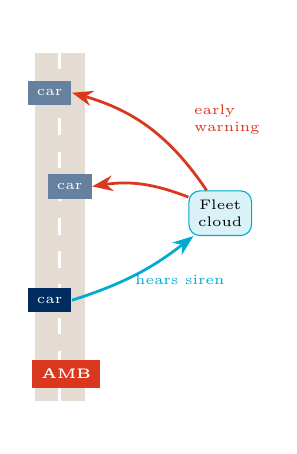
\begin{tikzpicture}[scale=0.85]
  \draw[line width=18pt,color=sand] (0,-2.6) -- (0,2.6);
  \draw[white,line width=1pt,dash pattern=on 6pt off 6pt] (0,-2.6) -- (0,2.6);
  \node[fill=alert,text=white,font=\tiny\bfseries,minimum width=0.5cm,minimum height=0.3cm] (amb) at (0.1,-2.2) {AMB};
  \node[fill=navy,text=white,font=\tiny,minimum width=0.45cm] (c1) at (-0.15,-1.1) {car};
  \node[fill=navy!60,text=white,font=\tiny,minimum width=0.45cm] (c2) at (0.15,0.6) {car};
  \node[fill=navy!60,text=white,font=\tiny,minimum width=0.45cm] (c3) at (-0.15,2.0) {car};
  \node[draw=sky,fill=sky!15,rounded corners,font=\tiny,align=center] (cl) at (2.4,0.2) {Fleet\\cloud};
  \draw[-{Stealth},sky,line width=1pt] (c1.east) to[bend right=10] node[font=\tiny,right,pos=0.4]{hears siren} (cl);
  \draw[-{Stealth},alert,line width=1pt] (cl) to[bend right=15] (c2.east);
  \draw[-{Stealth},alert,line width=1pt] (cl) to[bend right=20] (c3.east);
  \node[font=\tiny,alert,align=left] at (2.5,1.6) {early\\warning};
\end{tikzpicture}
\end{column}
\end{columns}
\end{frame}

% ================= FEASIBILITY =================
\begin{frame}{What Makes It Possible}
\vspace{-0.3cm}
\begin{columns}[T]
\begin{column}{0.48\textwidth}
\begin{block}{Only one new part}
4 small exterior microphones. Low-cost parts, and automotive-grade versions already exist for other exterior-microphone features.
\end{block}
\vspace{10pt}
\begin{block}{Everything else is already in the car}
\begin{itemize}
  \item Infotainment computer runs the AI
  \item Cabin speakers play the directional cue
  \item Instrument cluster shows the arrow
  \item Connected-car modem shares sirens
\end{itemize}
\end{block}
\end{column}
\begin{column}{0.48\textwidth}
\begin{block}{Runs inside the car, offline}
\begin{itemize}
  \item \textbf{Fast:} about 1 second from sound to alert, while a siren is audible hundreds of metres away
  \item \textbf{Private:} no audio is stored or leaves the car
  \item \textbf{Works in dead zones:} no network needed except for the optional fleet relay
  \item \textbf{Upgradeable:} improves through over-the-air updates
\end{itemize}
\end{block}
\vspace{6pt}
{\footnotesize\color{muted} A technical deep-dive is available on request.}
\end{column}
\end{columns}
\end{frame}

% ================= NOVELTY =================
\begin{frame}{What Exists, and What Is New}
\footnotesize\renewcommand{\arraystretch}{1.2}
\begin{tabularx}{\textwidth}{@{}p{4.3cm}YY@{}}
\toprule
\textbf{Prior work} & \textbf{What it does} & \textbf{Honk-Sense goes further} \\
\midrule
Siren detection and localisation patents (e.g. Motional) & Detect siren, estimate bearing, mainly for autonomous driving & Built for \emph{human} occupants, with tiered alerts \\
Sound-direction cabin feedback patent (US10351148B2) & Haptic or audio cue for direction & Adds India-specific classes and \emph{silence by default} \\
Horn/siren detection research (e.g. Forum Acusticum 2025) & Compares interior and exterior mics; stationary car & Works while driving, in wind and rain \\
Indian horn-detection projects & Noise policing in silence zones & In-vehicle driver assistance \\
\bottomrule
\end{tabularx}
\vspace{4pt}
\begin{block}{Our three novel elements}
\begin{enumerate}\small
  \item \textbf{India-trained sound understanding}: two-wheeler, auto, pressure horns and Indian sirens.
  \item \textbf{Alert-fatigue-first design}: deciding what \emph{not} to announce is the core feature.
  \item \textbf{Fleet siren relay}: cars that hear an ambulance warn the cars ahead of it. {\tiny\color{muted}(No production car in India found with this, Oct 2026.)}
\end{enumerate}
\end{block}
\end{frame}

% ================= BUSINESS =================
\begin{frame}{Value for Hyundai}
\vspace{-0.3cm}
\begin{columns}[T]
\begin{column}{0.48\textwidth}
\begin{block}{For customers}
\begin{itemize}
  \item Calmer, less stressful city driving
  \item Safer lane changes around two-wheelers
  \item Inclusive: helps hearing-impaired and elderly drivers
\end{itemize}
\end{block}
\vspace{3pt}
\begin{block}{For society}
\begin{itemize}
  \item Ambulances get through faster
  \item Anonymised honk-density maps could help cities target noise hot-spots
\end{itemize}
\end{block}
\end{column}
\begin{column}{0.48\textwidth}
\begin{block}{For Hyundai}
\begin{itemize}
  \item A visible, India-first feature, easy to demonstrate in showrooms
  \item Mostly software on existing hardware: scales across the line-up
  \item Fits connected-car subscriptions (fleet siren relay)
\end{itemize}
\end{block}
\end{column}
\end{columns}
\vspace{2pt}
\begin{center}

\begin{tikzpicture}
  \node[fill=navy,text=white,rounded corners=4pt,inner sep=7pt,font=\normalsize] {Mostly software, on hardware the car already has.};
\end{tikzpicture}
\end{center}
\end{frame}

% ================= ROADMAP =================
\begin{frame}{Roadmap}
\vspace{4pt}
\centering
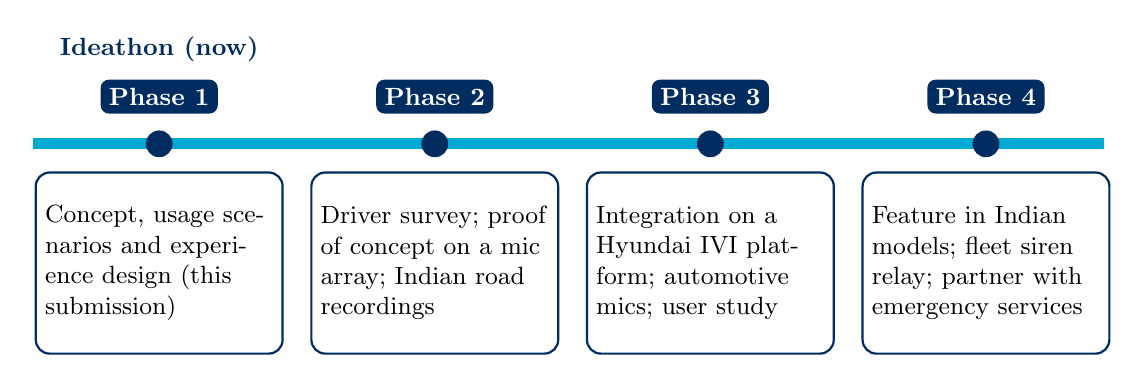
\begin{tikzpicture}[
  ph/.style={rectangle,rounded corners=5pt,text width=2.9cm,minimum height=2.3cm,align=left,font=\small,draw=navy,fill=white,line width=0.8pt},
  hd/.style={font=\small\bfseries,text=white}]
  \draw[line width=4pt,sky] (0,0) -- (13.6,0);
  \foreach \x/\t/\d/\b in {
    1.6/Phase 1/Ideathon (now)/{Concept, usage scenarios and experience design (this submission)},
    5.1/Phase 2//{Driver survey; proof of concept on a mic array; Indian road recordings},
    8.6/Phase 3//{Integration on a Hyundai IVI platform; automotive mics; user study},
    12.1/Phase 4//{Feature in Indian models; fleet siren relay; partner with emergency services}}{
    \fill[navy] (\x,0) circle (0.17);
    \node[hd,fill=navy,rounded corners=3pt,inner sep=3pt] at (\x,0.6) {\t};
    \node[font=\small\bfseries,navy] at (\x,1.2) {\d};
    \node[ph,anchor=north] at (\x,-0.35) {\b};
  }
\end{tikzpicture}
\end{frame}

% ================= REFERENCES =================
\newcommand{\refhead}[1]{\par\vspace{4pt}{\footnotesize\bfseries\color{navy}#1}\par\vspace{1pt}}
\newcommand{\refitem}[2]{\item #1 {\color{muted}\url{#2}}}
\setbeamertemplate{enumerate item}{\color{navy}\insertenumlabel.}

\begin{frame}{References}
\vspace{-0.2cm}
\fontsize{6.5}{7.8}\selectfont
\setlength{\itemsep}{0pt}
\refhead{Road safety and emergency response in India}
\begin{enumerate}\setlength{\itemsep}{0.5pt}
  \refitem{MoRTH, \emph{Road Accidents in India 2023} (PTI report).}{https://www.dtnext.in/news/national/172-lakh-people-died-in-480-lakh-road-accidents-in-2023-road-ministry-report-844831}
  \refitem{Collision-type shares, 2023 (MoRTH via PTI).}{https://theprint.in/economy/not-wearing-seat-belts-claimed-16025-lives-in-road-accidents-in-2023-morth/2731093}
  \refitem{Time to reach a health-care facility among road traffic accident victims, Puducherry.}{https://www.amrita.edu/publication/time-to-reach-health-care-facility-and-hospital-exit-outcome-among-road-traffic-accident-victims-attending-a-tertiary-care-hospital-puducherry/}
  \refitem{\emph{Too little, too late: emergency services require urgent care}, Deccan Herald.}{https://www.deccanherald.com/india/too-little-too-late-emergency-services-require-urgent-care-1216452.html}
\end{enumerate}
\refhead{Traffic noise and sirens}
\begin{enumerate}\setcounter{enumi}{4}\setlength{\itemsep}{0.5pt}
  \refitem{\emph{The levels and effects of traffic noise: a study in Mumbai} (IIT Bombay).}{https://www.audiology-worldnews.com/awareness/1844-the-levels-and-effects-of-traffic-noise-a-study-in-mumbai-india}
  \refitem{MPCB sub-group minutes on noise standards (horn and siren measurements).}{https://mpcb.gov.in/sites/default/files/internal-study-groups/Minutes_2ndMeetingSub\%20Group_noise\%20standards_siren.pdf}
  \refitem{Lok Sabha answer on ambient noise monitoring by CPCB.}{https://eparlib.nic.in/bitstream/123456789/803506/1/AU2897.pdf}
  \refitem{US DOT siren audibility study, summarised in JEMS.}{https://www.jems.com/ems-operations/ground-ambulance-operations/why-motorists-dont-get-out-way-0/}
\end{enumerate}
\end{frame}

\begin{frame}{References}
\vspace{-0.2cm}
\fontsize{6.5}{7.8}\selectfont
\refhead{Driver behaviour, blind spots and ADAS}
\begin{enumerate}\setcounter{enumi}{8}\setlength{\itemsep}{0.5pt}
  \refitem{Cicchino (IIHS), \emph{Effects of blind spot monitoring systems on lane-change crashes}, Traffic Injury Prevention, 2018.}{https://iihs.org/topics/bibliography/ref/2143}
  \refitem{\emph{Lane change behavior with a side blind zone alert system} (SWOV).}{https://swov.nl/en/publicatie/lane-change-behavior-side-blind-zone-alert-system}
  \refitem{FMCSA, inadequate surveillance and lane-change crashes.}{https://webarchive.library.unt.edu/web/20161101172143/https://cms.fmcsa.dot.gov/safety/driver-safety/cmv-driving-tips-inadequate-surveillance}
  \refitem{Texas Instruments, ultrasonic versus radar sensing (SPRY331).}{https://www.ti.com/lit/pdf/spry331}
  \refitem{Kumbhar and Pyasi, \emph{ADAS features in Indian driving conditions}, SAE 2026-26-0035.}{https://trid.trb.org/View/2761739}
\end{enumerate}
\refhead{Acoustic sensing and prior work}
\begin{enumerate}\setcounter{enumi}{13}\setlength{\itemsep}{0.5pt}
  \refitem{Detection of horns and sirens with interior vs exterior microphones, Forum Acusticum 2025.}{https://dael.euracoustics.org/confs/fa2025/data/articles/000006.pdf}
  \refitem{US10351148B2: sound direction detection in a vehicle.}{https://patents.google.com/patent/US10351148}
  \refitem{US 11804239: detection, classification and localisation of siren signals (Motional).}{https://patents.justia.com/patent/11804239}
  \refitem{US 2022/0180895: determining directionality of sounds detected by a vehicle.}{https://patents.justia.com/patent/20220180895}
  \item Knapp \& Carter (1976), generalized correlation method for time-delay estimation (GCC-PHAT), IEEE Trans. ASSP. Datasets: UrbanSound8K (2014), ESC-50 (2015), AudioSet (2017).
\end{enumerate}
\refhead{Photo credits (Wikimedia Commons)}
Ambulance, Kolkata: Biswarup Ganguly (CC BY 3.0) \textbullet\ Pune two-wheeler traffic: Amityadav8 (public domain) \textbullet\ Blow Horn: Justin Morgan (CC BY-SA 2.0) \textbullet\ Hairpin bend, Western Ghats: Rohini (CC BY-SA 3.0) \textbullet\ Traffic in Bangalore: Divya Chinnasamy (CC0)
\end{frame}

% ================= THANK YOU =================
{
\setbeamertemplate{footline}{}
\begin{frame}[plain]
\begin{tikzpicture}[remember picture,overlay]
  \fill[navy] (current page.south west) rectangle (current page.north east);
  \node[white,align=center] at (current page.center) {%
    {\fontsize{34}{36}\selectfont\bfseries Thank you}\\[14pt]
    {\Large\color{sky} Honk-Sense: the car hears what matters, so you don't have to}\\[24pt]
    {\small Piyush Anand \quad\textbullet\quad Ankith Deegoju \quad\textbullet\quad IIT Hyderabad}};
\end{tikzpicture}
\end{frame}
}

\end{document}
